\documentclass{altsu-bachelor}
\linespread{1,5}

\begin{document}

\begin{titlepage}
 \begin{center}
    \normalsize
    МИНИСТЕРСТВО НАУКИ И ВЫСШЕГО ОБРАЗОВАНИЯ \\
    РОССИЙСКОЙ ФЕДЕРАЦИИ \\
    ФГБОУ ВО «АЛТАЙСКИЙ ГОСУДАРСТВЕННЫЙ УНИВЕРСИТЕТ»
    \vfill
     
    Институт цифровых технологий, электроники и физики (ИЦТЭФ) \\
    Кафедра вычислительной техники и электроники (ВТиЭ)
    \vfill
     
    \textbf{Анализ характеристик выполнения параллельных приложений в виртуальной среде MPI-машины на примере работы тестовой программы вычисления числа $\pi$}
    
    Отчет по лабораторной работе №1
 \end{center}
\vfill
 
\newlength{\ML}
\settowidth{\ML}{«\underline{\hspace{3cm}}»}
\hfill\begin{minipage}{0.41\textwidth}
  Выполнил: студент гр. 5.306M\\
  \underline{\hspace{\ML}} А.\,В.~Лаптев \\
  Проверил: ст. преп. кафедры ВТиЭ\\
  \underline{\hspace{\ML}} И.\,А.~Шмаков \\
  «\underline{\hspace{1cm}}» \underline{\hspace{3cm}} \the\year г.
\end{minipage}%
\vfill
 
\begin{center}
  Барнаул, \the\year г.
\end{center}
\end{titlepage}

\setcounter{page}{2}

\textbf{Цель работы}

Изучить зависимости <<коэффициента ускорения>> и <<латентности>> вычислений на <<сетевой распределенной ВС>> по результатам вычислительных экспериментов, реализуемых с помощью тестовой параллельной MPI-программы по вычислению числа $\pi$.

\textbf{Задание}

\begin{enumerate}
    \item изучить стандарт интерфейса MPI (библиотекe функций как расширение системы программирования С/C++) – описание стандарта находится в Приложении к лабораторной работе в виде файла <<стандарт\_MPI\_Воеводин.doc>>;

    \item по приведенному ниже тексту MPI-программы восстановить алгоритм вычисления числа  и его блок-схему; для проведения вычислительных экспериментов в приложении имеется файл <<icpi.с>> c исходным текстом программы и исполняемый файл <<cpi.exe>>;

    \item провести вычислительные эксперименты, построить графики и диаграммы, оформить отчет.
\end{enumerate}

\textbf{Выполнение работы}

После знакомства со стандартом интерфейса и изучением приведенного в приложении кода был составлен алгоритм работы программы, на основании которого была создана блок-схема.

\textbf{Изменения исходного кода}

Изначально, для автоматизации программы для расчета значения числа $\pi$ для различного количества интервалов была частично переписана программа на языке C и также написан bash-скрипт, который является оберткой, в которой выполняется исполняемый файл заданное количество раз с заданными начальными условиями.

Текст измененной программы и bash-скрипт приведены в Приложении.

\textbf{Описание алгоритма}

\begin{enumerate}
    \item \textit{Начало}
    
    \item Инициализация MPI, определение числа процессов и номера текущего процесса.
    
    \item \label{algo1:input}Прочитать число интервалов для расчёта числа $\pi$.
    
    \item Фиксация времени начала вычислений для определения их скорости.

    \item \textit{Начало цикла}
    
    \item Для всех значений интервалов в счетчике вычислить аргумент подынтегральной функции.
    
    \item Для всех значений интервалов в счетчике вычислить значение подынтегральной функции.
    
    \item Для всех значений интервалов в счетчике прибавить значение к аккумулятору суммы.

    \item \textit{Конец цикла}
    
    \item Вычислить значение $mypi$ для каждого процесса.
    
    \item Сложить значения $mypi$ всех процессов в переменной $pi$ процесса с номером 0.
    
    \item Если номер процесса -- 0, зафиксировать время завершения вычислений и вывести значения:
    
    \begin{itemize}
        \item полученное значение числа $\pi$;
    
        \item ошибку вычисления числа $\pi$;
        
        \item время выполнения вычислений в секундах.
    \end{itemize}
    
    \item Возврат к шагу \ref{algo1:input}.
    
    \item Завершить работу процесса MPI.
    
    \item \textit{Конец}
\end{enumerate}

\textbf{Блок-схема алгоритма}

На рис.~\ref{fig:mpi} представлена блок-схема по приведенному выше алгоритму.

\begin{figure}[H]
    \centering
    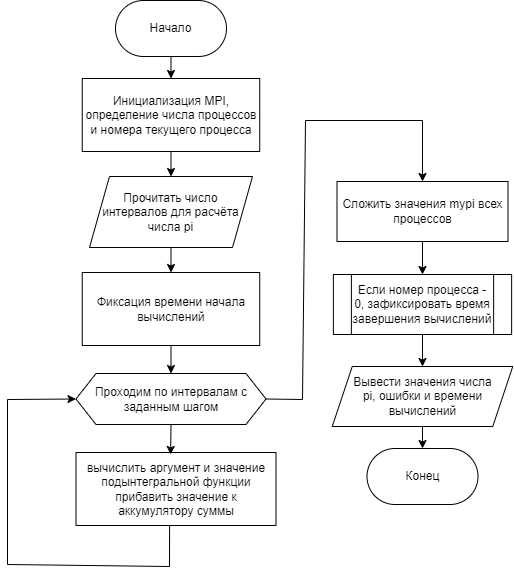
\includegraphics[scale=0.8]{icpi_block.png}
    \caption{Блок-схема алгоритма для расчета числа $\pi$}
    \label{fig:mpi}
\end{figure}

\textbf{Обработка результатов работы программы}

В результате работы программы был сформирован текстовый файл со всеми необходимыми исходными данными для построения графиков.

Ниже будет представлено несколько графиков, которые отображают зависимость различных параметров, используемых в расчетах друг от друга.

\begin{figure}[H]
    \centering
    \includegraphics{}
    \caption{Зависимость погрешности вычисления числа $\pi$ от числа интервалов}
    \label{fig:error}
\end{figure}

Для расчета следующей зависимости требуется найти ускорение, с которым обрабатываются одни и те же данные на разном количестве компьютеров. Это можно сделать по формуле:

$k_i = \frac{t_1}{t_i}$.

\begin{figure}[H]
    \centering
    \includegraphics{}
    \caption{\centering Коэффициент ускорения при вычислении числа $\pi$ на разном количестве компьютеров}
    \label{fig:speed}
\end{figure}

\begin{figure}[H]
    \centering
    \includegraphics{}
    \caption{Зависимость времени счета от количества интервалов}
    \label{fig:time}
\end{figure}

\textbf{Вывод}

Анализ вычислительных экспериментов показывает, что с увеличением в составе <<сетевой распределенной ЭВМ>> числа процессоров за счет увеличения обменов сообщениями между процессорами по <<комбинаторному закону>> увеличивается латентность в процессе выполнения параллельной программы (увеличиваются временные задержки), что приводит к снижению пропорционального роста ускорения вычислений.

\newpage
\chapter*{\begin{flushright}Приложение\end{flushright}}
\addcontentsline{toc}{chapter}{Приложение}

\begin{code}
\captionof{listing}{\label{code:icpi}Исходный код для расчета числа $\pi$}
\vspace{0.5cm}
{\small
\inputminted[mathescape,linenos,frame=lines,breaklines]{C++}{icpi.c}
}
\end{code}

\begin{code}
\captionof{listing}{\label{code:bash}Bash-скрипт для запуска исполняемого файла}
\vspace{0.5cm}
{\small
\inputminted[mathescape,linenos,frame=lines,breaklines]{C++}{bash_for_icpi}
}
\end{code}

\end{document}
